\documentclass{beamer}
\usepackage{tikz}
% overlay-beamer-styles is the library from the aobs-tikz package
\usetikzlibrary{overlay-beamer-styles, positioning}

\tikzset{
  highlight/.style={red, ultra thick},
  system/.style={
    draw, rectangle, rounded corners=3pt,
    minimum width=2cm, text width=1.8cm, align=center,
    outer sep=1pt, % fixed, so thick borders don't move the anchors
  },
}

\begin{document}
\begin{frame}
  \centering
  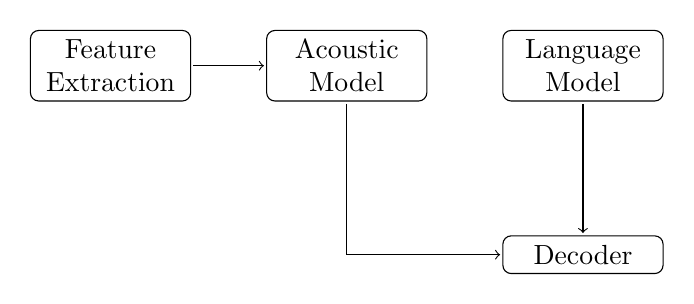
\begin{tikzpicture}[node distance=2.4cm and 3cm, on grid]
    \node [system, alt=<3->{highlight}{}] (fe) {Feature Extraction};
    \node [system, alt={<2,4>{green}{}}, right=of fe]
      (am) {Acoustic Model};
    \node [system, right=of am,
           alt=<-2>{blue}{}, alt=<3>{highlight}{}, alt=<4>{green}{}]
      (lm) {Language Model};
    \node [system, below=of lm] (d) {Decoder};

    \draw [->] (fe) -- (am);
    \draw [->] (am) |- (d);
    \draw [->] (lm) -- (d);

    % pin the bounding box, so beamer doesn't re-center a picture
    % that grew because of a thick border
    \pgfresetboundingbox
    \useasboundingbox (fe.north west) rectangle (lm.east |- d.south);
  \end{tikzpicture}
\end{frame}
\end{document}
